\graphicspath{{chapters/01/}}
\chapter{Evolution of single cell}

\hypertarget{the-history-of-sequencing}{%
\section{The history of sequencing}\label{the-history-of-sequencing}}

The history of sequencing begins in the 1950s with the first sequenced
protein (Insulin) by Fred Sanger. The term ``bioinformatics'' first
appears in 1979. From the 2000s, the Human Genome Project allows to
`crack the code' and sequencing costs dramatically reduce going towards
2010 with third generation sequencing. Data analysis becomes a central
topic in genome studies, since sequencing requires a huge amount of data
management. The majority of biological data is stored by:

\begin{itemize}
\tightlist
\item
  NCBI (USA)
\item
  SIB (Switzerland)
\item
  EBI (Europe)
\item
  BIG (China)
\item
  DDBJ (Japan)
\end{itemize}

\hypertarget{analysis-of-gene-expression-in-single-neurons-1992}{%
\subsection{Analysis of gene expression in single neurons
(1992)}\label{analysis-of-gene-expression-in-single-neurons-1992}}

The first two single cell articles focus on the characterization of
single neuron gene expression in rat hippocampus and cerebellum,
respectively. They applied two similar techniques:

\begin{itemize}
\tightlist
\item
  \textbf{in vitro transcription},  which amplifies the original material
  linearly through a transcription reaction
\item
  \textbf{PCR},  to obtain an exponential increase in transcripts
\end{itemize}

\hypertarget{analysis-of-gene-expression-in-single-live-neurons-ivt}{%
\subsubsection{\texorpdfstring{\textbf{Analysis of gene expression in
single live neurons
(IVT)}}{Analysis of gene expression in single live neurons (IVT)}}\label{analysis-of-gene-expression-in-single-live-neurons-ivt}}

Quotes from the paper:

``The RNA from \textbf{defined single cells} is amplified by
microinjecting primer, nucleotides, and enzyme into acutely dissociated
cells from a defined region of rat brain.''

``We demonstrate this method by constructing expression profiles of
single live cells from rat hippocampus''.

``This profiling suggests that cells that appear to be morphologically
similar may show marked differences in patterns of expression.''

\hypertarget{ampa-receptor-subunits-expressed-by-single-purkinje-cells}{%
\subsubsection{AMPA receptor subunits expressed by single Purkinje
cells}\label{ampa-receptor-subunits-expressed-by-single-purkinje-cells}}

\textbf{Purkinje cells} are a class of GABAergic inhibitory neurons
located in the cerebellum. It was possible to determine the subset of
AMPA receptor subunits expressed by single cerebellar Purkinje cells in
culture by combining whole-cell patch-clamp recordings and a molecular
analysis, based on PCR, of the messenger RNAs harvested into the pipette
at the end of each recording.

\hypertarget{single-cell-transcriptional-analysis-of-neuronal-progenitors-2003}{%
\subsection{Single-cell transcriptional analysis of neuronal progenitors
(2003)}\label{single-cell-transcriptional-analysis-of-neuronal-progenitors-2003}}

Single cell analysis by \textbf{microarray} in the olfactory system,
which is composed of well-characterized cells in terms of shape and
differentiation stages (e.g.~olfactory progenitors (OPCs) and mature
sensory neurons (OSNs)) → ideal system to test. The material was
amplified with PCR and analyzed through an Affymetrix microarray.

\begin{tcolorbox}
[width=\linewidth, sharp corners=all, colback=white!95!black]

\textbf{RQ: }\emph{Find the number of genes that were used:} 
Affymetrix Mu11K high-density oligonucleotide arrays containing 13027 probe sets.
\end{tcolorbox}

\begin{figure}
\centering
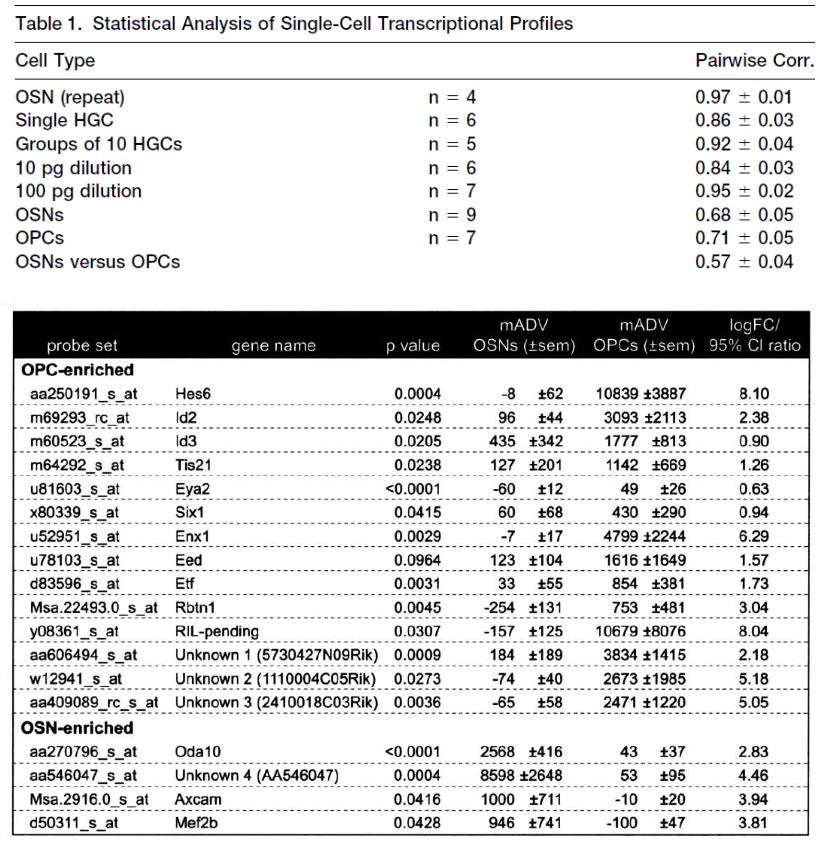
\includegraphics[width=0.4\textwidth]{images/Screenshot_2023-03-15_at_11-30-24.png}
\caption{\emph{Tietjen I. et al.~Single-cell transcriptional analysis of
neuronal progenitors. Neuron. 2003 Apr 24;38(2):161-75.}}
\end{figure}

Example of statistical analysis, quantification of correlation:

\begin{itemize}
\tightlist
\item
  technical repeat with OSN cell to tune the system
\item
  measure the correlation among different cell types; variation could be
  due to stochasticity, biological variation (rather than technical)
\end{itemize}

Quotes from the paper:

``To uncover mechanisms involved in neuronal differentiation and
diversification, we have monitored the expression profiles of
\textbf{individual neurons and progenitor cells} collected from
dissociated tissue or laser captured from intact brain slices.''

``This technique provides a sensitive and reproducible
\textbf{representation of the single-cell transcriptome}.''

``In the olfactory system, hundreds of transcriptional differences were
identified between olfactory progenitors (OPCs) and mature sensory
neurons (OSNs), enabling us to define the large variety of signaling
pathways expressed by individual progenitors at a precise developmental
stage.''

\hypertarget{mrna-seq-whole-transcriptome-analysis-of-a-single-cell-2009}{%
\subsection{mRNA-Seq whole-transcriptome analysis of a single cell
(2009)}\label{mrna-seq-whole-transcriptome-analysis-of-a-single-cell-2009}}

\hypertarget{method}{%
\subsubsection{Method}\label{method}}

The single cell is manually picked under a microscope and lysed. Then
mRNAs are reverse-transcribed into cDNAs using a poly(T) primer with
anchor sequence (UP1) and unused primers are digested. Poly(A) tails are
added to the first-strand cDNAs at the 3' end, and second-strand cDNAs
are synthesized using poly(T) primers with another anchor sequence
(UP2). Then cDNAs are evenly amplified by PCR using UP1 and UP2 primers,
fragmented, and P1 and P2 adaptors are ligated to the ends.

\begin{figure}
\centering
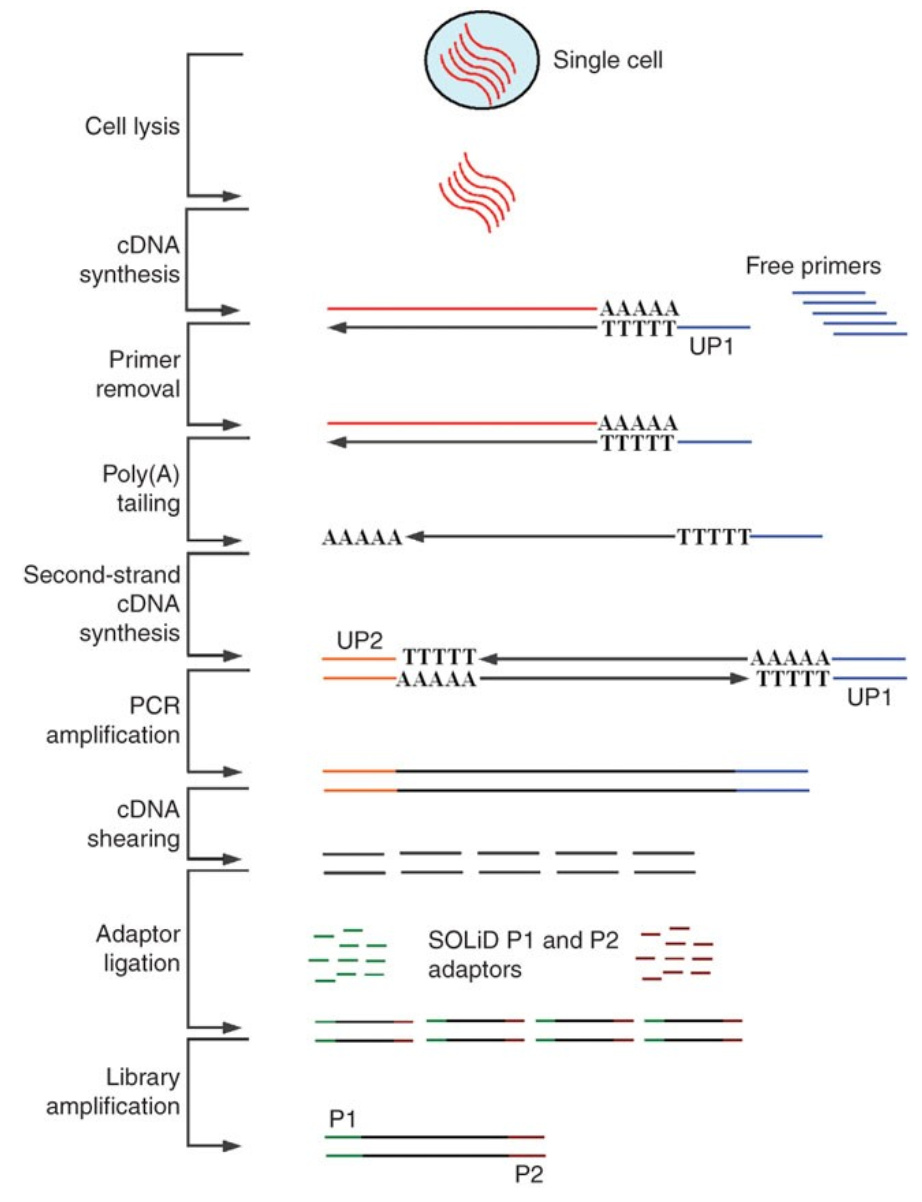
\includegraphics[width=0.3\textwidth]{images/Screen_Shot_2023-02-20_at_19-18-51.png}
\caption{\emph{Tang, F. et al.~mRNA-Seq whole transcriptome analysis of
a single cell. Nat Methods \textbf{6,} 377--382 (2009)}}
\end{figure}

\hypertarget{results}{%
\subsubsection{\texorpdfstring{\textbf{Results}}{Results}}\label{results}}

More than 100 million 35-base reads and 50-base reads were obtained from
the cRNA expression profile of a single mouse blastomere. The method
detected the expression of 75\% (5,270) more genes than microarray
techniques and identified 1,753 previously unknown splice junctions
called by at least 5 reads.

\textbf{Coverage plots}: determine whether mRNA-Seq assay could be used
to dissect the functional consequences when one of the critical genes
for microRNA synthesis,~\emph{Dicer1}, was conditionally knocked out
during oocyte development. The reads were found in exons with sharp
boundaries at the exon-intron junction, confirming the single-exon
resolution of the mRNA-Seq reads. This demonstrated that the single cell
mRNA-Seq assay is accurate and has low or even no background noise.

\textbf{Pros:}

\begin{itemize}
\tightlist
\item
  increasing the cDNA length up to 3 kb by extending the incubation time
  for reverse transcription allows to capture full-length cDNAs for the
  majority of expressed genes.
\item
  the assay can be used to discover new transcripts and alternative
  splicing isoforms.
\item
  detect low-level transcripts - important for early embryo studies
  because some of the key transcription factors are expressed at very
  low levels
\end{itemize}

\textbf{Cons:}

\begin{itemize}
\tightlist
\item
  mRNAs without poly(A) tails, such as histone mRNAs, will not be
  detected by our mRNA-Seq assay
\item
  for most of the mRNAs longer than 3 kb, the 5' end that is more than 3
  kb away from the 3' end of the mRNA will not be detected
\item
  the assay uses double-stranded cDNAs but cannot discriminate between
  sense and antisense transcripts
\end{itemize}

\hypertarget{characterization-of-the-single-cell-transcriptional-landscape-by-highly-multiplex-rna-seq-2011}{%
\subsection{Characterization of the single-cell transcriptional
landscape by highly multiplex RNA-seq
(2011)}\label{characterization-of-the-single-cell-transcriptional-landscape-by-highly-multiplex-rna-seq-2011}}

\hypertarget{methods}{%
\subsubsection{Methods}\label{methods}}

Isolated single cells were barcoded individually in a 96-well plate,
then transferred into a single tube, called \emph{single-cell tagged
reverse transcription sequencing} (STRT-seq), for PCR amplification. The
amplified samples were then adapted for Illumina sequencing.

The feasibility of the strategy was demonstrated by analyzing the
transcriptomes of 85 single cells collected from two different mouse
cell types: embryonic stem cells (ES) and embryonic fibroblasts (MEFs).

\hypertarget{results-1}{%
\subsubsection{Results}\label{results-1}}

Single-cell RNA-seq expression profiles were clustered to form a
two-dimensional cell map onto which expression data were projected.
Three levels of organization are depicted: the whole population of
cells, the functionally distinct subpopulations it contains, and the
single cells themselves.

\begin{figure}
\centering
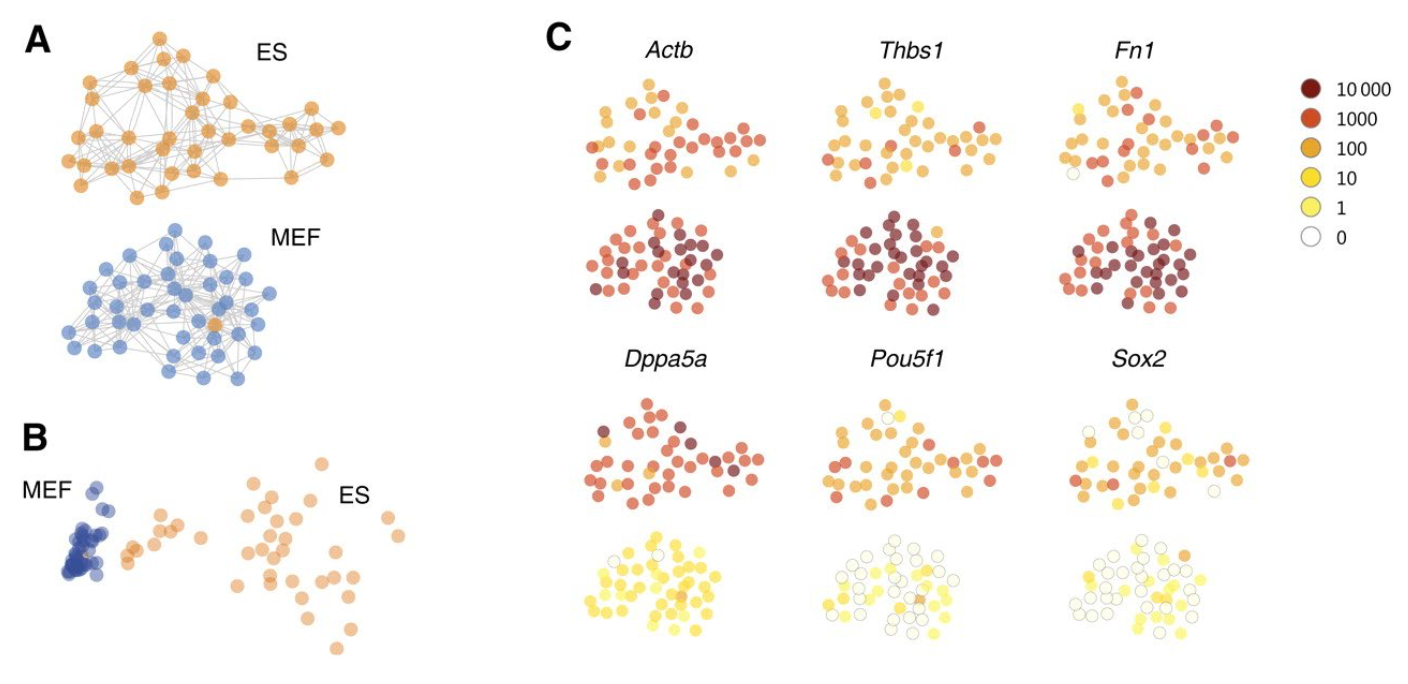
\includegraphics[width=0.5\textwidth]{images/Screen_Shot_2023-02-20_at_19-24-40.png}
\caption{\emph{Islam et al.~Genome Res. 2011}}
\end{figure}

\begin{tcolorbox}
[width=\linewidth, sharp corners=all, colback=white!95!black]

\textbf{RQ: }\emph{How did the authors quantify the similarity between cells in panel
A?}

In the two-dimensional map, more closely related cells are located near
each other, so as to be able to detect and distinguish cell types based
solely on expression data. In the underlying graph, the nodes represent
cells and edges represent cell-to-cell similarity of expression pattern.
Raw reads were normalized to TPM - obtained by counting the number of
hits to each annotated gene and normalizing the data to transcripts per
million. The similarity measure was computed through the Bray-Curtis
distance, which handles the noise in low-expressed genes better than
standard correlation.
\end{tcolorbox}


\begin{itemize}
\item
  Bray-Curtis dissimilarity

  Is a statistic used to quantify the compositional dissimilarity
  between two different sites, based on counts at each site.

  \(BC_{ij}=1-\frac{2C_{ij}}{S_i+S_j}\)

  Where \(C_{ij}\) is the sum of the lesser values (see example below)
  for only those species in common between both sites. \(S_i\) and
  \(S_j\) are the total number of specimens counted at both sites.

  The Bray--Curtis dissimilarity is bounded between 0 and 1, where 0
  means the two sites have the same composition (that is they share all
  the species), and 1 means the two sites do not share any species. It
  is not a distance since it does not satisfy triangle inequality, and
  should always be called a dissimilarity to avoid confusion.
\end{itemize}

\hypertarget{cel-seq-single-cell-rna-seq-by-multiplexed-linear-amplification-2012}{%
\subsection{CEL-Seq: Single-Cell RNA-Seq by Multiplexed Linear
Amplification
(2012)}\label{cel-seq-single-cell-rna-seq-by-multiplexed-linear-amplification-2012}}

Study of early \emph{C. elegans} embryonic development at single-cell
resolution. Differential distribution of transcripts between sister
cells is seen as early as the two-cell stage embryo, and zygotic
expression in the somatic cell lineages is enriched for transcription
factors.

\hypertarget{methods-1}{%
\subsubsection{Methods}\label{methods-1}}

\begin{figure}
\centering
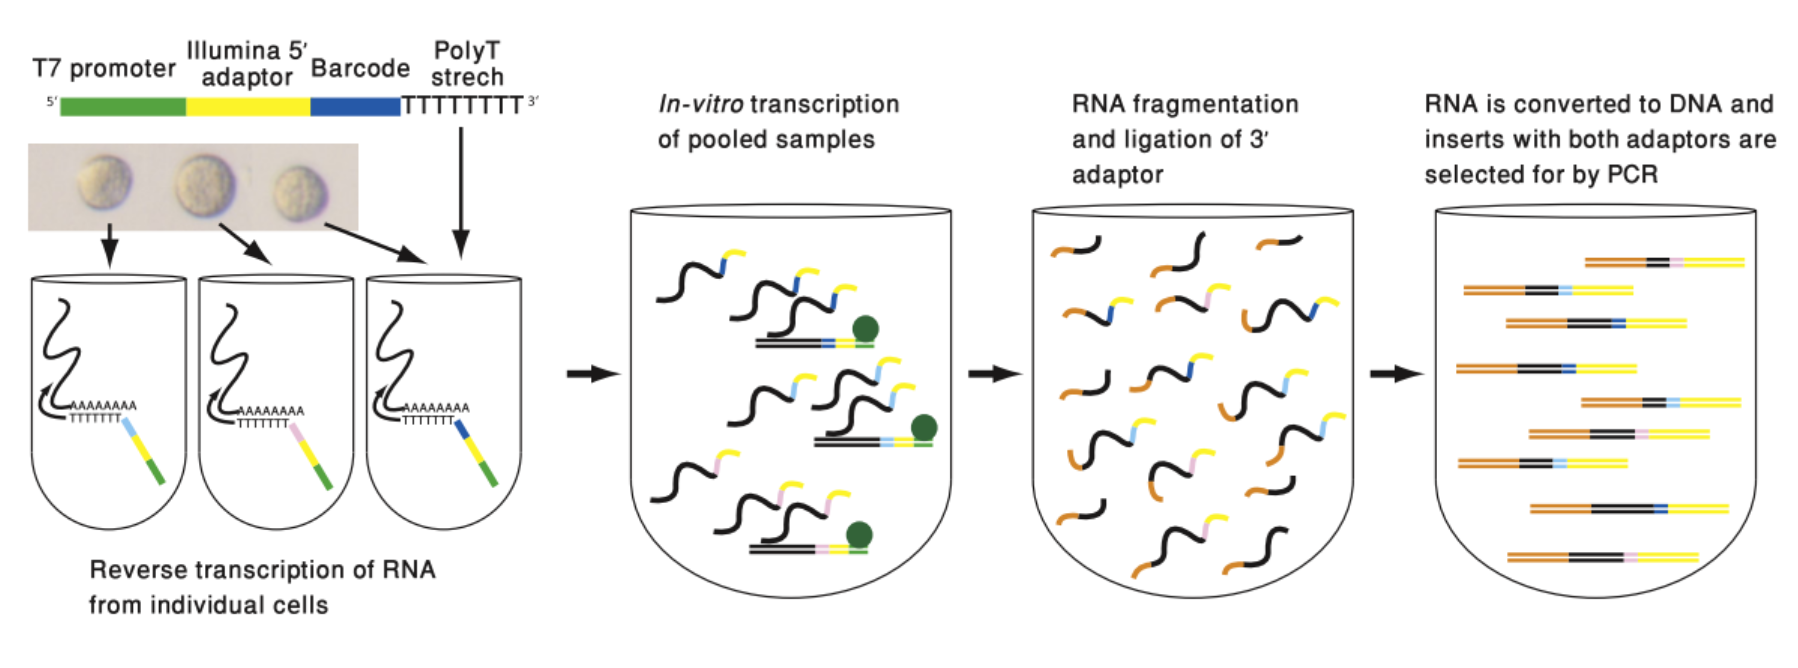
\includegraphics[width=0.5\textwidth]{images/Screen_Shot_2023-02-21_at_13-19-47.png}
\caption{Hashimshony  et al., Cell Rep,2012}
\end{figure}

Individual cells are added to tubes, each with a uniquely bar-coded
primer for reverse transcription. After second-strand synthesis, the
reactions are pooled for IVT. The amplified RNA is then fragmented and
purified before entry into a modified version of the Illumina
directional RNA protocol, the molecules with both Illumina adaptors are
selected, and the DNA library is sequenced with paired-end reads.

\begin{tcolorbox}
[width=\linewidth, sharp corners=all, colback=white!95!black]

\textbf{RQ: }\emph{Did the authors compare CEL-seq to STRT-seq? If so, how?}

CEL-Seq was applied to the same cell types by Islam et al., 2011
(STRT-seq)

\begin{enumerate}
\def\labelenumi{\arabic{enumi}.}
\tightlist
\item
  compare the distribution of expression levels of each single-cell
  transcriptome across methods and cell type → CEL-Seq shows more
  reproducible distributions of expression, higher correlations for ES
  cells and distinguishes between cell types more clearly
\item
  evaluate the amount of detected genes → CEL-Seq detects significantly
  more genes in the ES cells.
\item
  quantify reproducibility for each method separately → with CEL-Seq,
  significantly lower noise was detected across biological replicates
  for both cell types tested.
\item
  compare PCA → principal component analysis based on CEL-Seq data
  better distinguishes between cell types than the corresponding STRT
  data
\end{enumerate}
\end{tcolorbox}

\hypertarget{results-2}{%
\subsubsection{Results}\label{results-2}}

CEL-Seq can be used to identify biological differences between closely
related cells in the~\emph{C.~elegans} embryo.~\emph{C.~elegans}
embryonic development begins with unequal cleavages producing founder
cells---termed blastomeres. The AB and P1 sister blastomeres were
examined 10 min after cell division → 17 genes with a mean 2-fold
difference showing significantly different expression.

\begin{figure}
\centering
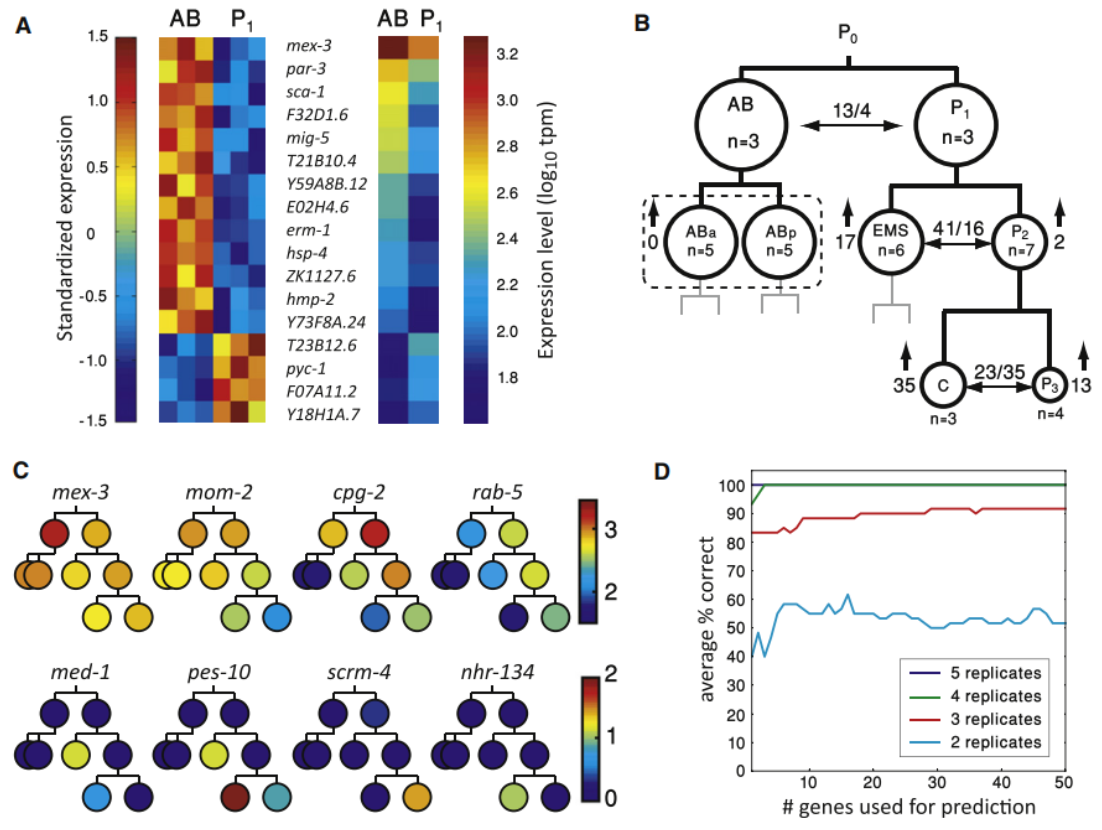
\includegraphics[width=0.5\textwidth]{images/Screen_Shot_2023-02-20_at_19-30-17.png}
\caption{\emph{Hashimshony et al.~Cell Rep.~2012}}
\end{figure}

\begin{enumerate}
\def\labelenumi{(\Alph{enumi})}
\tightlist
\item
  Differential expression analysis between AB and P1
\item
  The blastomeres examined in the study, with numbers of new transcripts
  and differential transcripts between anterior and posterior
  blastomeres.
\item
  Gene expression levels (log10 tpm; see color scale on right) for the
  indicated genes; cell lineage is as in (B).
\item
  Classification performance of the AB and P1 blastomeres.
\end{enumerate}


\textbf{Pros:}

\begin{itemize}
\tightlist
\item
  ability to harness the power of IVT, providing both multiplexing and
  reproducibility
\item
  reduced hands-on time both for the amplification and downstream
  processing, allowing for the preparation of dozens of samples for
  sequencing within 2--3 days
\item
  commercially available kits for the amplification and sequencing
  library preparation → cost effective
\end{itemize}

\textbf{Cons:}

\begin{itemize}
\tightlist
\item
  mRNAs without poly(A) tails, such as histone mRNAs, will not be
  detected by our mRNA-Seq assay
\item
  for most of the mRNAs longer than 3 kb, the 5' end that is more than 3
  kb away from the 3' end of the mRNA will not be detected
\item
  the assay uses double-stranded cDNAs but cannot discriminate between
  sense and antisense transcripts
\end{itemize}

\hypertarget{smart-seq}{%
\subsection{SMART-seq}\label{smart-seq}}

\hypertarget{full-length-mrna-seq-from-single-cell-levels-of-rna-and-individual-circulating-tumor-cells-2012}{%
\subsubsection{Full-length mRNA-Seq from single-cell levels of RNA and
individual circulating tumor cells
(2012)}\label{full-length-mrna-seq-from-single-cell-levels-of-rna-and-individual-circulating-tumor-cells-2012}}

``Compared with existing methods, Smart-Seq has improved read coverage
across transcripts, which enhances detailed analyses of alternative
transcript isoforms and identification of single-nucleotide
polymorphisms. The assay was applied to putative circulating tumor cells
(CTCs) captured from the blood of a melanoma patient''.

\begin{figure}
\centering
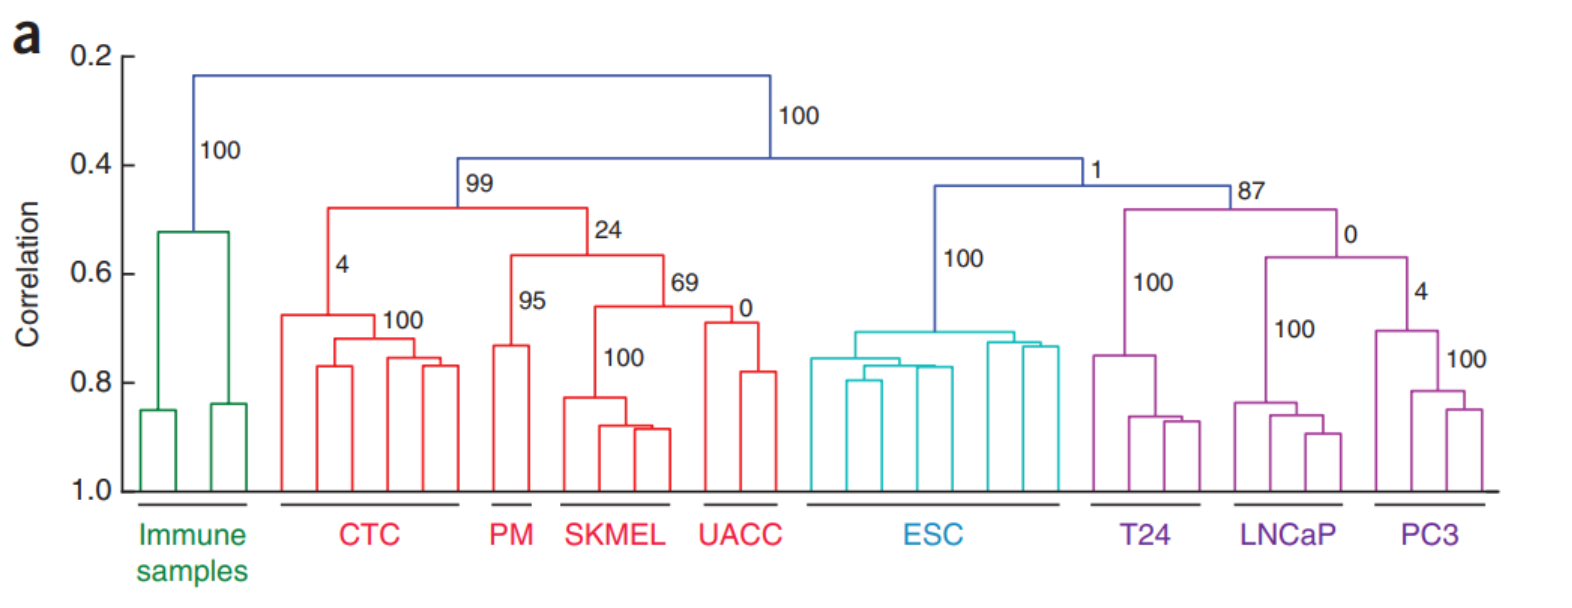
\includegraphics[width=0.5\textwidth]{images/Screen_Shot_2023-02-21_at_19-30-18.png}
\caption{\emph{Ramskold et al, et al.~Nature Biotech 2012}}
\end{figure}

Clustering of single cell transcriptomes, based on expression of highly
expressed genes (\textgreater100 RPKM). Confidence in clusters are
indicated. Samples analyzed: human immune samples cells from putative
melanoma CTCs (CTC), primary melanocytes (PM), melanoma cell lines
SKMEL5 (SKMEL) and UACC257 (UACC), prostate cancer cell lines (LNCaP and
PC3), bladder cancer cell line (T24) and human embryonic stem cells
(ESC).

\hypertarget{smart-seq2-for-sensitive-full-length-transcriptome-profiling-in-single-cells-2013}{%
\subsubsection{Smart-seq2 for sensitive full-length transcriptome
profiling in single cells
(2013)}\label{smart-seq2-for-sensitive-full-length-transcriptome-profiling-in-single-cells-2013}}

Advantages:

\begin{itemize}
\tightlist
\item
  \textbf{High coverage} across transcripts (recovery of full-length
  cDNAs)
\item
  High level of mappable reads per cell (up to $10^6$)
\end{itemize}

Limitations:

\begin{itemize}
\tightlist
\item
  lack of strand specificity
\item
  inability to detect nonpolyadenylated (polyA) RNA
\item
  low number of cells ($< 10^3$)
\end{itemize}

\begin{tcolorbox}
[width=\linewidth, sharp corners=all, colback=white!95!black]

\textbf{RQ: } \emph{What is the important step to obtain full length coverage?}

\textbf{Template switching} allows for the capture of full cDNA
sequences, for which the 5' end is unknown, in a relatively sensitive
manner. Poly(A)+ RNA is converted to full-length cDNA using oligo(dT)
priming and SMART template switching technology. In addition, KAPA
preamplification improves cDNA generation, allowing for the detection of
more genes at higher GC levels and improved sensitivity and accuracy, as
well as read coverage.
\end{tcolorbox}

\hypertarget{single-cell-rna-counting-at-allele-and-isoform-resolution-using-smart-seq3-2020}{%
\subsubsection{Single-cell RNA counting at allele and isoform resolution
using Smart-seq3
(2020)}\label{single-cell-rna-counting-at-allele-and-isoform-resolution-using-smart-seq3-2020}}

Advantages:

\begin{itemize}
\tightlist
\item
  High coverage across transcripts (recovery of full-length cDNAs)
\item
  Suitable for \textbf{isoform}/allele analysis
\item
  High level of mappable reads per cell (up to $10^6$)
\end{itemize}

Limitations:

\begin{itemize}
\tightlist
\item
  inability to detect nonpolyadenylated (polyA) RNA.
\item
  low number of cells ($10^3,10^4$)
\end{itemize}

\hypertarget{method-of-the-year-2013}{%
\subsection{Method of the year (2013)}\label{method-of-the-year-2013}}

Single-cell sequencing was chosen by Nature as Method of the Year 2013.

``Technologies for single-cell amplification and sequencing are
maturing. As the cost and ease of examining individual cells improves,
the approach will enter the hands of more researchers as a standard tool
for understanding biology at high resolution''. The focus is on both RNA
and DNA single cell sequencing.

\hypertarget{drop-seq-2015}{%
\subsection{Drop-seq (2015)}\label{drop-seq-2015}}

A microfluidic device joins two aqueous flows. One contains cells, the
other contains barcoded primer beads. After compartmentalization into
discrete droplets, the cell is lysed and releases its mRNAs, which then
hybridize to the primers on the microparticle surface. The droplets are
broken and the microparticles collected and washed. The mRNAs are then
reverse-transcribed in bulk, forming STAMPs, and template switching is
used to introduce a PCR handle downstream of the synthesized cDNA.

\begin{figure}
\centering
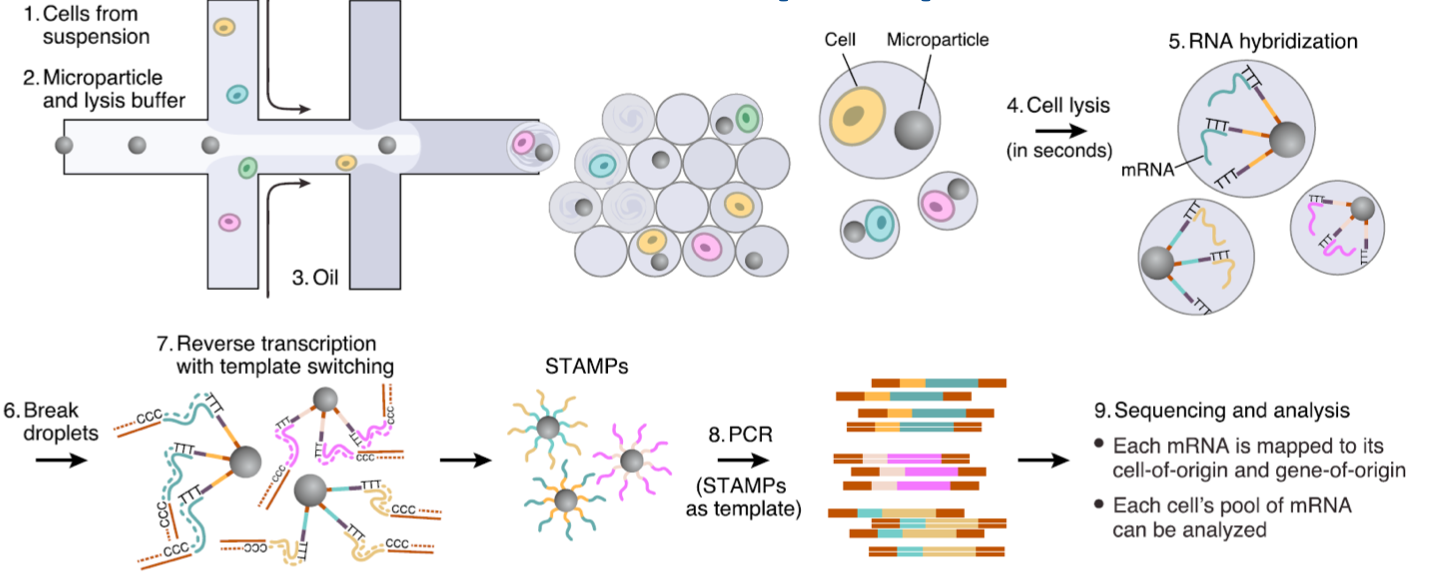
\includegraphics[width=0.5\textwidth]{images/Screen_Shot_2023-02-21_at_19-51-12.png}
\caption{Macosko et al., Cell 2015}
\end{figure}

\textbf{Barcoding:} sequence of primers on the microparticle. The
primers on all beads contain a common sequence (``PCR handle'') for PCR
amplification. Each microparticle contains more than $10^8$ individual
primers that share the same ``cell barcode'' but have different
\textbf{unique molecular identifiers} (UMIs), enabling mRNA transcripts
to be digitally counted. A 30-bp oligo dT sequence is present at the end
of all primer sequences for capture of mRNAs.

Pros:

\begin{itemize}
\tightlist
\item
  From hundreds to thousands cells ($10^4$)
\item
  3' end sequencing
\item
  Use of UMI (Unique Molecular Identifiers)
\end{itemize}

\hypertarget{umi}{%
\subsubsection{UMI}\label{umi}}

Unique Molecular Identifiers are composed of a randomized nucleotide
sequence (8-12 nt long) incorporated into the complementary DNA in the
initial steps of RNA-seq protocol before the subsequent amplification
steps. The goal of UMIs , in case of reads with identical cDNA sequence,
is to distinguish between:

\begin{itemize}
\tightlist
\item
  amplified copies of the same mRNA molecule (same cDNA sequence, same
  UMI → technical duplicates, removed)
\item
  reads from separate mRNA molecules transcribed from the same gene
  (same cDNA, different UMI → biological duplicates, kept)
\end{itemize}

UMIs reduce the amplification noise by allowing the removal of
amplification (PCR) duplicates.

\begin{figure}
\centering
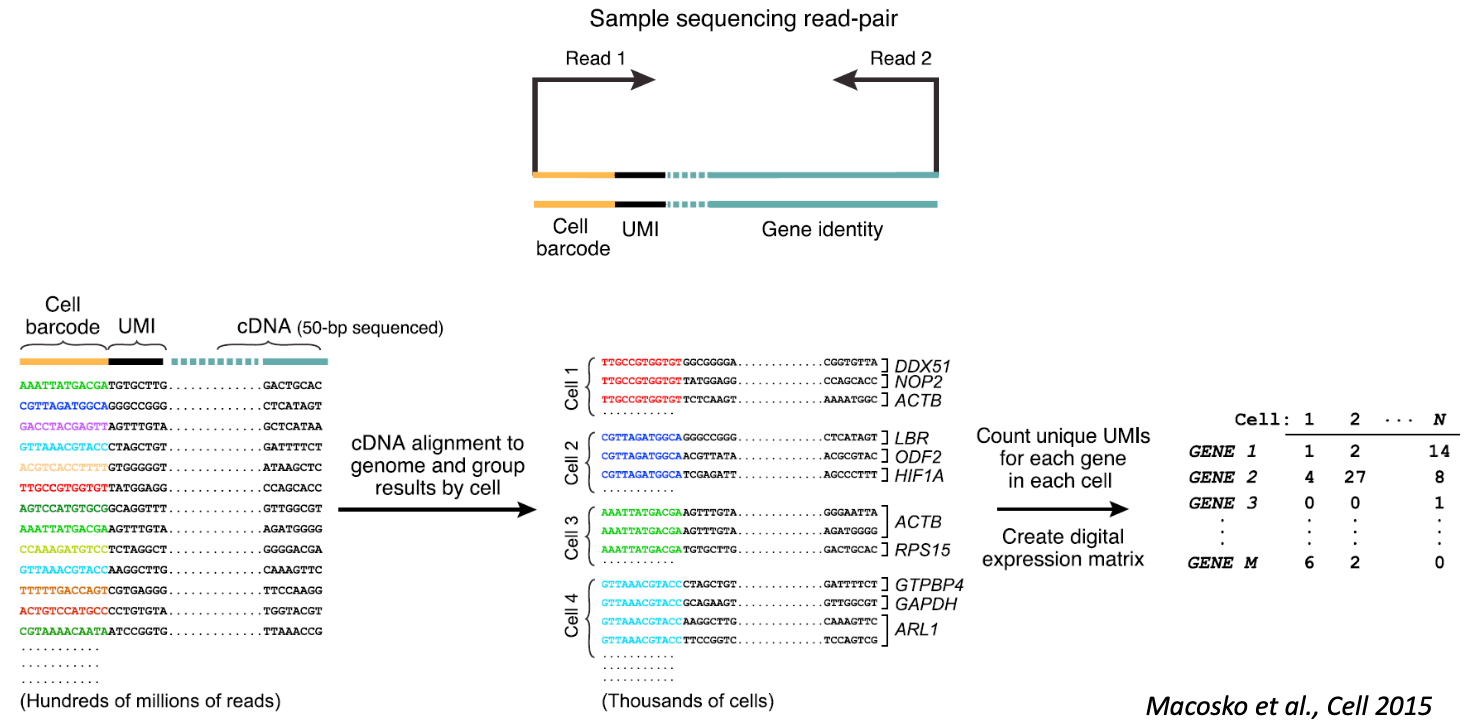
\includegraphics[width=0.5\textwidth]{images/Screen_Shot_2023-02-21_at_19-54-26.png}
\caption{Macosko et al., Cell 2015}
\end{figure}

\hypertarget{cell-cycle-analysis}{%
\subsubsection{Cell cycle analysis}\label{cell-cycle-analysis}}

Classification of cells based on the expression of \textbf{known cell
cycle genes.} A \textbf{phase-specific} score was calculated for each
cell across \textbf{five} phases from gene expression levels. Classic
cell cycle genes encompass CCNB1\&2, MCM2-7,MCM10, ARUKA and AURKB.

\hypertarget{analysis-of-the-mouse-retina-45k-cells}{%
\subsubsection{Analysis of the mouse retina (45k
cells)}\label{analysis-of-the-mouse-retina-45k-cells}}

Analysis of mouse retina, quite well known system - neurons with
distinct morphological features. From 45k cells, the authors performed
multidimensional scaling and reduction; they were able to identify 39
clusters with similar expression. The color of the clusters reflects
neuron type, based on known marker genes.

The expression of the markers is specific, visualized as a violin plot.

\begin{tcolorbox}
[width=\linewidth, sharp corners=all, colback=white!95!black]

\textbf{RQ: }
\emph{What are the computational tools used for the analysis?}

\begin{enumerate}
\def\labelenumi{\arabic{enumi}.}
\tightlist
\item
  PCA on STAMPs and tSNE
\item
  combined a density clustering approach with post hoc differential
  expression analysis to divide 44,808 cells among 39 transcriptionally
  distinct clusters
\item
  organized the 39 cell populations into larger categories (classes) by
  building a dendrogram (hierarchical clustering) of similarity
  relationships among the 39 cell populations
\end{enumerate}
\end{tcolorbox}

\hypertarget{indrop-device}{%
\subsubsection{inDrop device}\label{indrop-device}}

Droplet based approach, published on the same Cell issue containing the
Drop-seq paper. Each component has an inlet: RT mix, cells, DNA
barcoding hydrogels (at the left of the instrument) and oil (in the
middle). Cells and DNA barcoding hydrogels are then isolated in the
collection outlet.

\begin{figure}
\centering
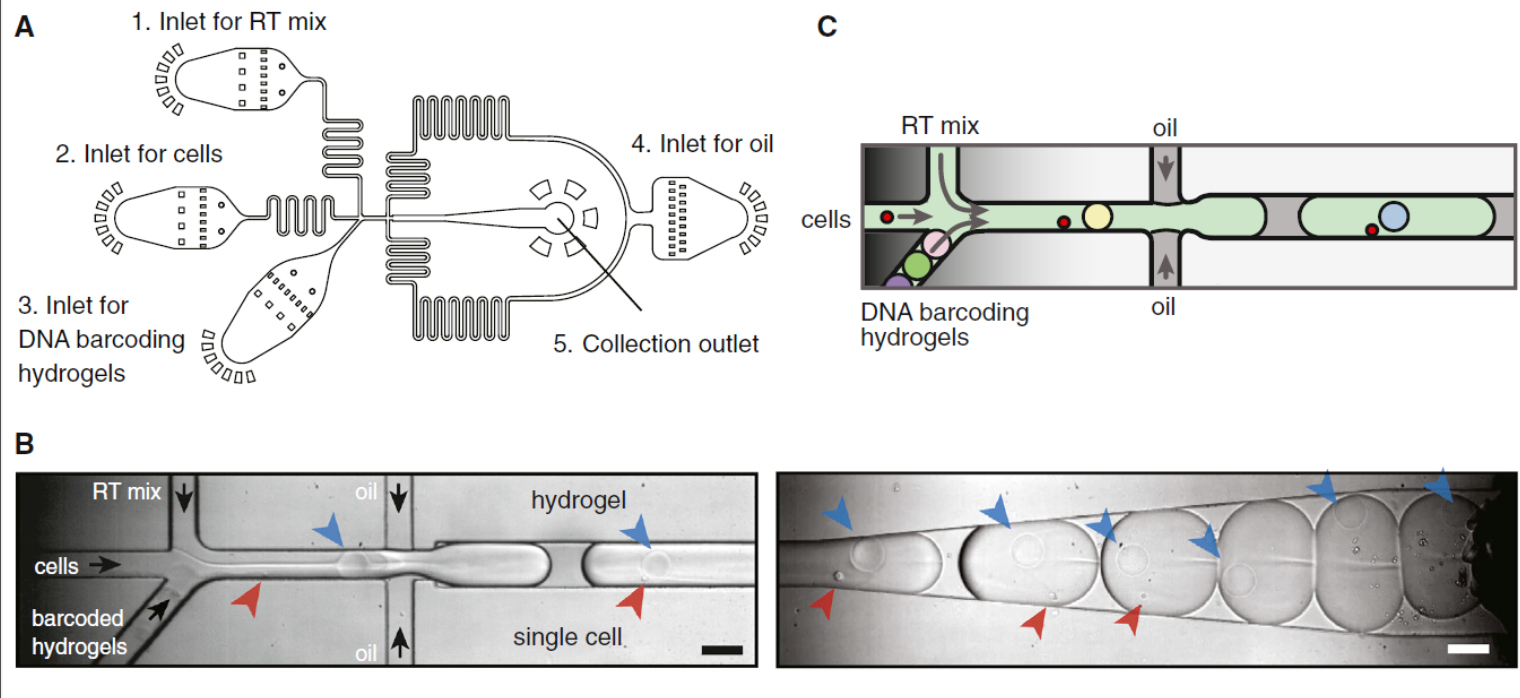
\includegraphics[width=0.5\textwidth]{images/Screen_Shot_2023-02-21_at_20-02-42.png}
\caption{\emph{Klein et al, Cell 2015}}
\end{figure}

Drop-seq can be applied for evaluating the heterogeneity in
differentiating ES cells.

Loadings of the components are useful to identify the expression of
genes having a major impact in characterizing clusters. Example: genes
connected with translation, elongation factors, cytoskeleton\ldots{}

\textbf{Analysis:} differentiation of embryonic stem cells after
leukemia inhibitory factor(LIF)withdrawal. ES cells maintained in serum
exhibit well-characterized fluctuations, but are uniform compared to
differentiated cell types and thus pose a challenge for single cell
sequencing. The differentiating ES cell population underwent significant
changes in population structure, qualitatively seen by hierarchical
clustering cells. In the first four principal components it was possible
to identify:

\begin{itemize}
\tightlist
\item
  one rare population (6/935 cells) with very low levels of pluripotency
  markers and high levels of PrEn markers
\item
  a second cell population (15/935 cells) expressed high levels
  of~\emph{Krt8},~\emph{Krt18},~\emph{S100a6, Sfn} and other markers of
  the epiblast lineage.
\item
  the third population represented a seemingly uncharacterized state,
  marked by expression of heat shock proteins~\emph{Hsp90},~\emph{Hspa5}
  and other ER components such as the disulphide isomerase~\emph{Pdia6}.
\end{itemize}

These sub-populations expressed low levels of pluripotency factors,
suggesting they are biased toward differentiation or have already exited
the pluripotent state. The latter population could also reflect stressed
cells.

They also visualized clusters at different stages in order to determine
subpopulation characterized by biomarkers. Some cells failed to express
epiblast markers and a fraction of these expressed pluripotency factors
at undifferentiated levels even seven days after LIF withdrawal → after
7 days, 5\% (\emph{N}=799) of cells overlapped with the ES cell
population.

\hypertarget{human-cell-atlas-2016}{%
\subsection{Human Cell Atlas (2016)}\label{human-cell-atlas-2016}}

International group of researchers (2,300 members, 83
countries) use a combination of single-cell and spatial omics
technologies to create \textbf{cellular reference maps} with the
position, function, and characteristics of \textbf{every cell type in
the human body}.

\hypertarget{x-genomics-2016-2017}{%
\subsection{10X Genomics (2016-2017)}\label{x-genomics-2016-2017}}

10x Technology samples a pool of \textasciitilde750,000 10x Barcodes to
separately index each cell's transcriptome. Next, barcoded gel beads are
mixed with cells, enzyme and partitioning oil (\textbf{Gel bead
emulsion}, GEM). Single cell GEMs undergo RT to generate 10x Barcoded
cDNA and all generated cDNA from individual cells share a common 10x
Barcode.

\begin{itemize}
\tightlist
\item
  \emph{Chromium}: this Next GEM technology enables the analysis of
  individual biological components at scale.
\item
  \emph{Visium}: spatial capture technology enabling the analysis of
  mRNA molecules within their morphological content.
\end{itemize}

Through Chromium, cell encapsulation of up to 8 samples at a time takes
place in 6 minutes, with 50\% cell capture efficiency.

Thanks to this technique, it is possible to detect distinct populations
in peripheral blood mononuclear cells. PBMC: remove cell without nuclei (erythrocytes and platelets)
and with multinuclei (granulocytes) to remain with lymphocytes (T cells, B cells, NK cells) and monocytes.

\hypertarget{genotype-and-single-cell-expression-analysis-of-transplant-bmmcs-bone-marrow-mononuclear-cells}{%
\subsubsection{``Genotype'' and single-cell expression analysis of
transplant BMMCs (Bone Marrow Mononuclear
Cells)}\label{genotype-and-single-cell-expression-analysis-of-transplant-bmmcs-bone-marrow-mononuclear-cells}}

Standard treatment in AML involves transplant from a healthy donor. The
analysis profiles bone marrow samples from AML patients and healthy
patients and compares profiles before and after transplant. The authors
built a method based on SNV identification able to distinguish cells
from donor and from host. The main idea involved checking whether the
transplant was modifying differentiation patterns in bone marrow; indeed
profiles are quite different and this confirmed the efficacy of the
treatment in restoring a healthy cell population, even though the
typical signature of AML persists.

\begin{figure}
\centering
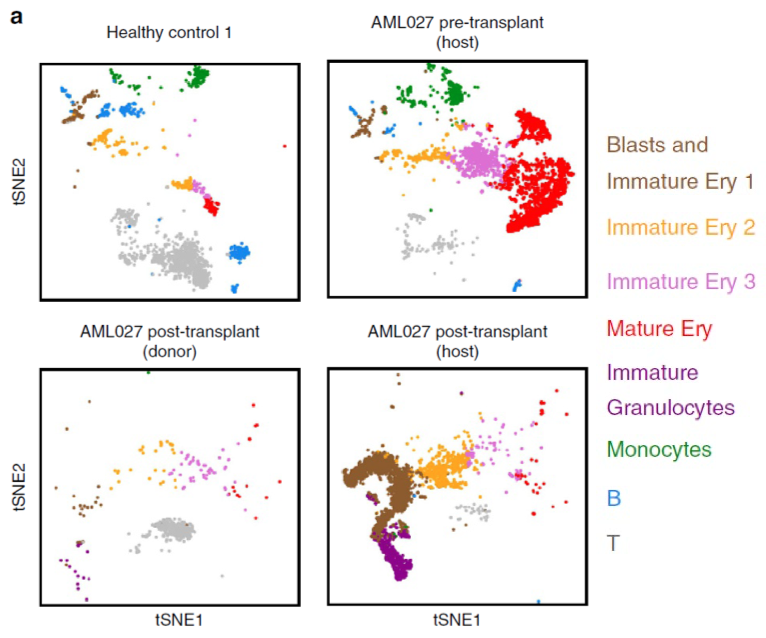
\includegraphics[width=0.5\textwidth]{images/Screenshot_2023-03-24_at_08-16-37.png}
\caption{\emph{Grace et al, Nat Comms 2017}}
\end{figure}

\hypertarget{split-seq-2018}{%
\subsection{SPLiT-seq (2018)}\label{split-seq-2018}}

\begin{itemize}
\tightlist
\item
  labels the cellular origin of RNA through \textbf{combinatorial
  barcoding}
\item
  compatible with fixed cells or nuclei
\end{itemize}

SPLiT-seq does not require partitioning single cells into individual
compartments (droplets, microwells, or wells) but relies on the cells
themselves as compartments.  The technique starts by passing a suspension of formaldehyde-fixed
cells or nuclei through four rounds of combinatorial barcoding in 96
wells plates. After sequencing, each transcriptome is assembled by
combining reads containing the same four-barcode combination (21M
barcode combinations).

\begin{enumerate}
\def\labelenumi{\arabic{enumi}.}
\tightlist
\item
  nuclei extraction
\item
  sample multiplexing
\item
  split-pool barcoding
\item
  clustering and visualization
\end{enumerate}

More than 150.000 nuclei from P2 and P11 mouse brains and spinal cords
were profiled in a single experiment employing more than 6 million
barcode combinations obtained from 4 rounds. Each cluster was then
downsampled to 1000 cells for visualization.

Astrocytes from different spots, while oligodendrocytes have a specific
shape → characterize subclusters in the differentiation process. By
looking at an isolated closeup, we can distinguish that immature cells
and mature cells are ordered in different positions on the tSNE. The
coordinate of differentiation is called \textbf{\emph{pseudotime}}. We
are required to manually insert the root of the trajectory to obtain a
reasonable trend.

\begin{figure}
\centering
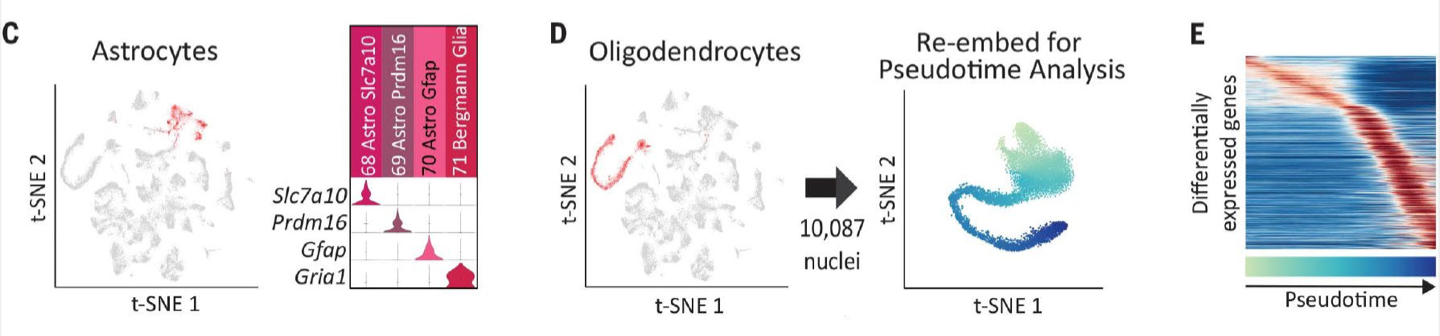
\includegraphics[width=0.5\textwidth]{images/Screenshot_2023-03-24_at_08-21-13.png}
\caption{\emph{Rosenberg et al, Science 2018}}
\end{figure}


\hypertarget{split-pool-barcoding}{%
\subsubsection{Split-pool barcoding}\label{split-pool-barcoding}}

In each split-pool round, fixed cells or nuclei are randomly distributed
into wells, and transcripts are labeled with well-specific barcodes.
Barcoded RT primers are used in the first round. Second- and third-round
barcodes are appended to cDNA through ligation. A fourth barcode is
added to cDNA molecules by PCR during sequencing library preparation.

\begin{figure}
\centering
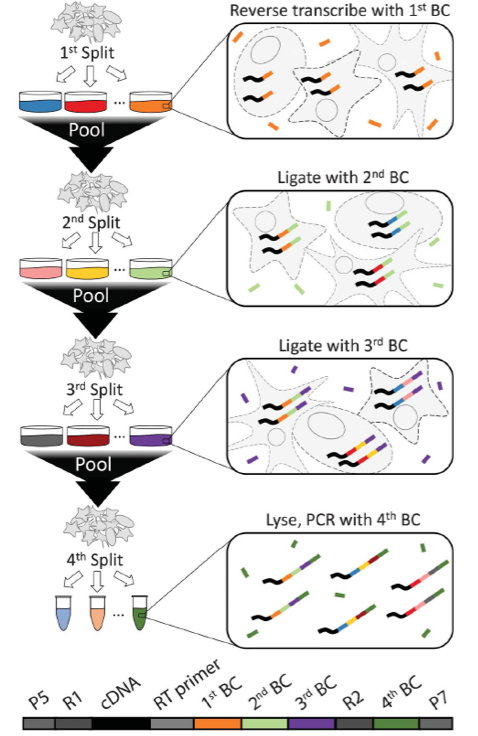
\includegraphics[width=0.3\textwidth]{images/Screenshot_2023-03-24_at_08-04-47.png}
\caption{\emph{Rosenberg et al, Science 2018}}
\end{figure}


\textbf{Pros:}

\begin{itemize}
\tightlist
\item
  fixation can reduce perturbations to endogenous gene expression during
  cell handling and makes it possible to store cells for future
  experiments
\item
  \textbf{the use of nuclei bypasses the need to obtain intact single
  cells}
\item
  may be used to profile single nuclei from formalin-fixed,
  paraffin-embedded tissue
\item
  the use of the first-round barcode as a sample identifier makes it
  possible to profile a large number and variety of samples in parallel,
  thus minimizing batch effects
\item
  efficient use of reagents
\end{itemize}

Critical aspect in droplet-based approaches: cells often associate with
multiple barcodes by multiple beads occurring within the same droplet or
heterogeneity of oligonucleotide sequences within a single bead.

\section{Comparison of scRNA-seq preparation}

\begin{figure}
\centering
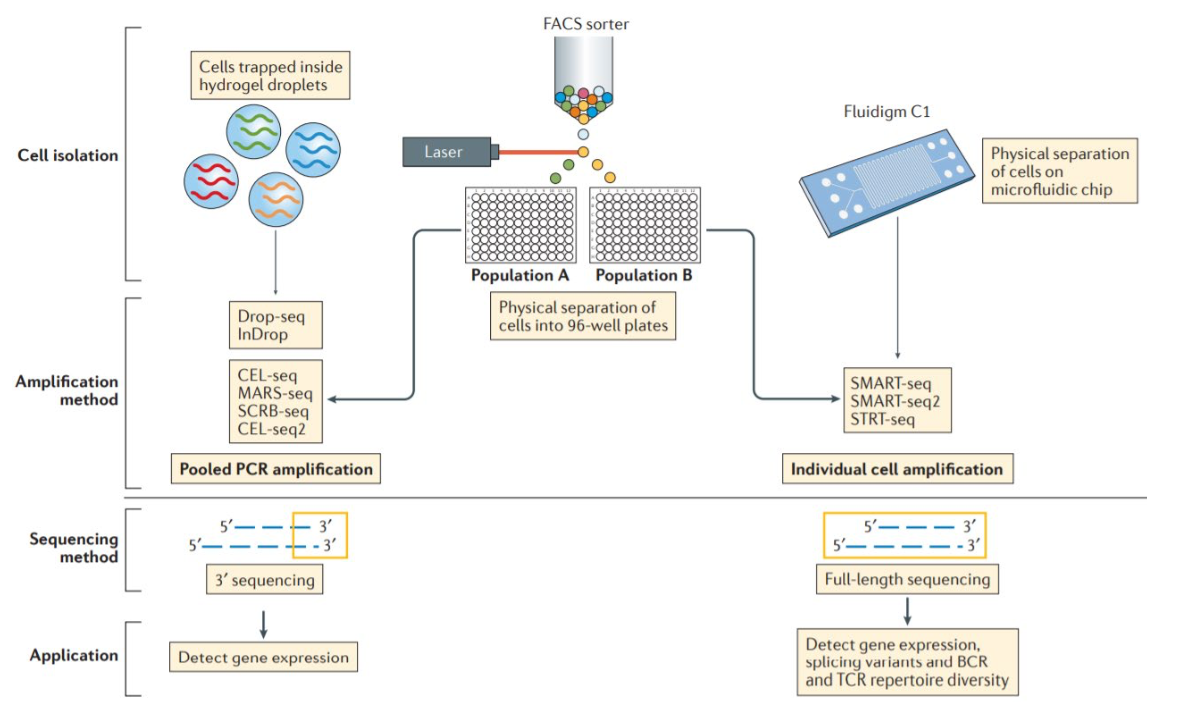
\includegraphics[width=0.5\textwidth]{images/Screen_Shot_2023-02-21_at_22-35-31.png}
\caption{\emph{Papalexi et al, Nat Rev Immunol. 2018}}
\end{figure}

\begin{figure}
\centering
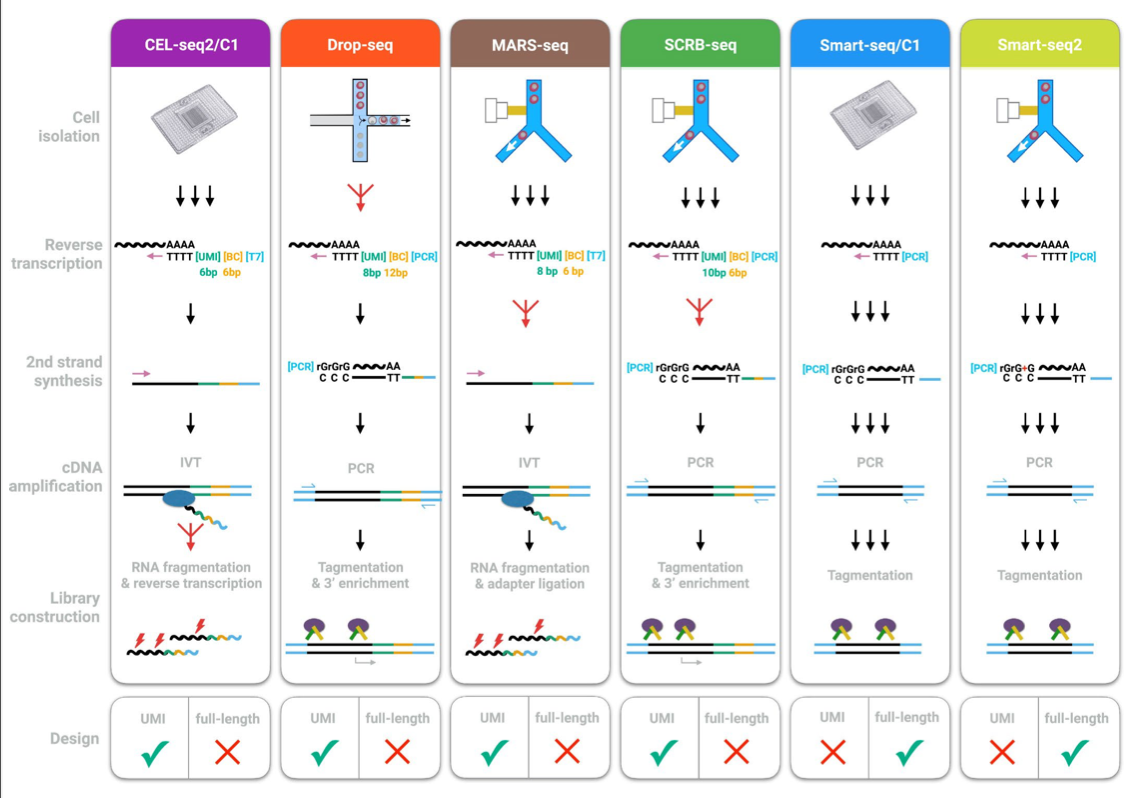
\includegraphics[width=0.5\textwidth]{images/Screen_Shot_2023-02-21_at_22-36-08.png}
\caption{\emph{Ziegenhaim et al, Mol Cell 2017}}
\end{figure}

\begin{figure}
\centering
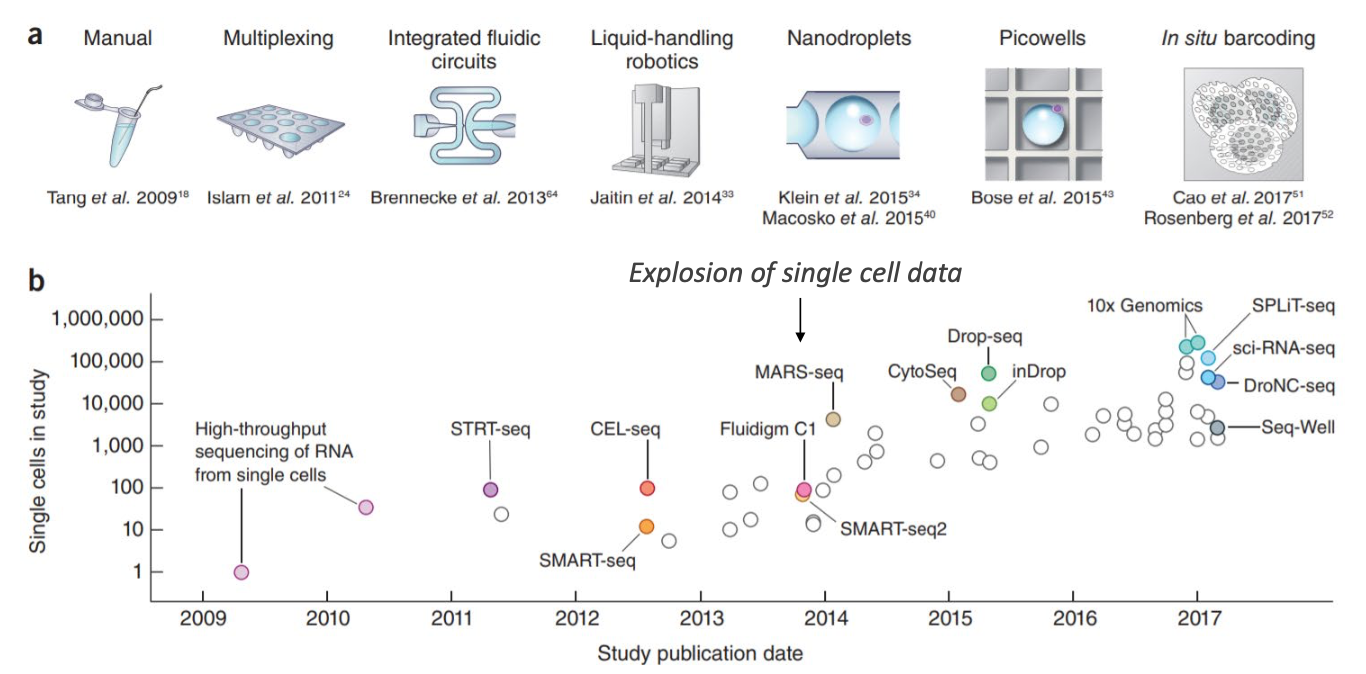
\includegraphics[width=0.5\textwidth]{images/Screen_Shot_2023-02-21_at_22-40-17.png}
\caption{Screen Shot 2023-02-21 at 22-40-17.png}
\end{figure}
